\documentclass[a4paper]{article}
\usepackage[english]{babel}
\usepackage[utf8]{inputenc}   
\usepackage{hyperref}
\usepackage{graphicx}
\usepackage{amsmath}
\usepackage{booktabs}
\usepackage{lipsum}

\renewcommand{\arraystretch}{1.5}

\graphicspath{ {./images/} }  
\bibliographystyle{plain} 

\title{ \Huge{Yamaha Aerox Sa14 Limiter Concept} }
\author{Kasper Ederzeel, Dylan Duunk}
\date{\today}

\begin{document}

\begin{titlepage}
    \maketitle
\end{titlepage}    

\pagenumbering{roman}

\newpage

\begin{abstract}
    \noindent
    Many people nowadays own a scooter.
    These scooters are often capable of reaching speeds of 60+ km/h.
    Those speeds are much higher than is permitted by the law.
    That is why the maximum speed of store bought scooters is limited to 45 km/h.
    \\ \\
    This is among others done with a vario ring.
    Many people choose to remove this vario ring so that the maximum speed of the scooter is over 45 km/h.
    The disadvantage of this is that you easily get caught speeding.
    Most of the times when you get caugt your scooter will be tested for the maximum speed of the scooter.
    You can bypass this by using a limiter, a limiter is a device that makes the scooter's maximum speed lower in certain circumstances.
    That way the scooter cannot drive faster than officially permitted.
    \\
    For example a limiter is controlled by plugging in a headphone jack or a flipping a switch. 

    \vspace{7px}
    \begin{center}
        \textit{''But what if you were to automate this process?''}
    \end{center}
\end{abstract}

\newpage
\tableofcontents
\newpage
\pagenumbering{arabic}

\nocite{*}

\section{Concept}
This is the idea: 
\\ \\
When a scooter is on the roller conveyor (a machine that measures the maximum speed of a scooter), only the rear wheel is on the roller conveyor.
The front wheel is standing still, this gives us the opportunity to check whether the front wheel is moving or not.
\\ \\
If the front wheel is not moving, the scooter is either on a roller conveyor or is standing still.
This is when you want the limiter to be on and the scooter to run at 45 km/h.
As soon as the front wheel starts moving for a set amount of time you can assume the scooter is moving.
This is when you want the limiter to be off and the scooter to run above 45 km/h.
\\ \\
A way of checking if the front wheel is moving is to use a sensor, in this case an hall-sensor on the front wheel.
If the signal of this sensor is above a threshold value for a set amount of time, we assume the scooter is moving.
If not we assume the scooter is either on a roller conveyor or standing still.
\\ 
This signal is processed by an Arduino, this is the brain of our limiter.
The Arduino check the signal of the hall-sensor and controls the limiter.
\\ \\ 
As of limiting the scooter we make use of an capacitor, in our case a 2.2$\mu F$ capacitor.
When connecting this capacitor between the signal wire from the CDI (see figure \ref{fig:cdi_pinout}) and the GND we limit the scooter to around 40 km/h.
\begin{figure}[h]
    \caption{CDI Pinout}
    \centering
    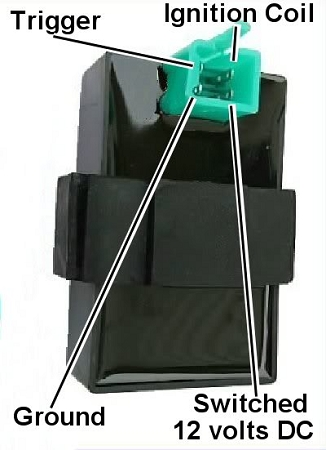
\includegraphics[scale=0.3]{CDI-Pinout.jpg}
    \label{fig:cdi_pinout}
\end{figure}
\\
If using a capacitor lower than 2.2$\mu F$ the scooter is limited to a lower km/h. 
When using a capacitor higher than 2.2$\mu F $ the scooter is limited to a higher km/h, eventually capping out on the maximum speed.
The connection between between the signal wire from the CDI and the GND can be controlled using a relay, this acts like a swith which can be controlled with the Arduino.
\\ \\
This makes the process of limiting a scooter automated.
\newpage

\bibliography{literature}

\end{document}
